\chapter{Introducción} \label{ch:introduction}

\section{Actividad eléctrica del corazón} \label{sec:electrical-activity}

\indent El corazón esta formado, su mayor parte, por tejido muscular que consta de células altamente diferenciadas
para la función contráctil que forman las paredes de las cámaras auriculares y ventriculares. El resto está
organizado en estructuras específicas implicadas en la generación y propagación de impulsos eléctricos. La actividad
eléctrica comienza a nivel de células que generan de manera espontánea potenciales de acción, llamadas
\textit{células marcapaso}. Esta propiedad se encuentra más o menos desarrollada en diversas zonas del tejido
especializado. El grupo celular que posee la frecuencia intrínseca más elevada es el \textit{nódulo sinoauricular}
(Keith, Flack. 1907 \cite{pp:keith_flack}), que constituye el marcapaso primario del corazón. Su frecuencia de
descarga \textit{in situ} es de alrededor de 1.25 Hz (75 impulsos por minuto). Situado a nivel de la unión de la
vena cava superior y la aurícula derecha, está formado por un grupo de miocitos ramificados que se conectan con las
células del miocardio auricular. De importancia fisiológica es el hecho de que las células del nódulo sinusal están
sometidas a una acción de estiramiento que puede modular su frecuencia de descarga. Este estiramiento sería inducido
por la presencia de la arteria del nódulo sinusal y por la distensión de las paredes de la aurícula durante el
arribo de sangre proveniente de las venas cavas. \\
\indent El \textit{nódulo auriculoventricular}, localizado en el piso de la aurícula derecha, entre el seno
coronario y la válvula tricúspide, contiene células similares a las del nódulo SA, pero su frecuencia intrínseca de
descarga es menor. La parte superior contiene células de transición. Éstas generan un potencial lento, de poca
amplitud, que se conduce a muy baja velocidad. La lenta conducción del impulso a través del nódulo AV engendra un
retardo entre la activación auricular y la ventricular, lo que permite una contracción secuencial de estas cámaras.
Las fibras inferiores del nódulo AV convergen y forman el \textit{haz de His}. Las ramas del haz de His terminan en
las \textit{fibras de Purkinje}, cuyas propiedades eléctricas les confieren la mayor velocidad de conducción. Estas
células forman una red subendocárdica, a partir de la cual transmiten el influjo eléctrico al músculo ventricular.
El sistema de Prukinje asegura la casi sincrónica activación de toda la masa ventricular desde el endocardio al
epicardio y desde el ápex hacia la base.

\subsection{El potencial de acción cardíaco} \label{subsec:action-potential}

El potencial cardíaco se define como la polarización y despolarización de la membranas de las células
miocárdicas. Esto produce una diferencia de potencial trasmembranal que sirve para transmitir información entre
células. Es producido por la llegada de un impulso eléctrico a la célula de modo que produce una redistribución
de carga que genera estas diferencias de potenciales. Estos cambios derivan de la apertura y cierre subsecuente
de los canales iónicos según una cinética particular para cada uno. El fenómeno de excitación dura alrededor de
0.5 ms en la fibra nerviosa, 5-10 ms en la fibra muscular esquelética y 250 ms en la fibra cardíaca ventricular.
La bomba de $Na^+$-$K^+$ no desempeña ningún papel directo en la generación del potencial de acción, ya que su
función se limita al mantenimiento de los gradientes de $Na^+$ y $K^+$, mientras que el gradiente de $Ca^{2+}$ es
mantenido por las bombas de $Ca^{2+}$ situadas en la membrana celular y en la del retículo sarcoplasmático. \\
\indent Este fenómeno se encuentra compuesta de 5 fases distinguibles que ayudan a mantener el potencial de
acción. Cabe aclarar que este potencial de acción son las células del miocardio ya que las células marcapasos poseen
un funcionamiento claramente diferente. En la Figura \ref{fig:action_potential_phases} se ilustra estas etapas.

\begin{itemize}
  \item \textbf{Fase 0}: \textbf{corriente de sodio ($I_{Na}$)}. La fase 0 constituye la despolarización rápida del
  potencial de acción. En las células ventriculares, así como en las células auriculares y de la red de His-Purkinje,
  esta rápida despolarización depende de la apertura de los \textit{canales rápidos de $Na^+$} similares a los
  presentes en el músculo esquelético y el nervio. Esta corriente de $Na^+$ ($I_{Na}$) es designada como rápida porque
  exhibe cinética de activación e inactivación muy rápida en comparación con otras corrientes.
  Debido a que los canales rápidos de $Na^+$ son operados por voltaje, luego de la despolarización la compuerta
  de \textit{activación} se abre y $I_{Na}$ llega a su pico en aproximadamente 1 ms. Luego de la activación pico
  de $I_{Na}$ la corriente comienza a disminuir debido al cierre de los canales mediante el proceso de
  \textit{inactivación}, que en este caso se debe a la interacción del extremo aminoterminal de la proteína
  que forma el canal con el poro de éste (inactivación de tipo N). Por lo tanto, $I_{Na}$ es prácticamente cero en
  pocos milisegundos. Una vez que el canal se encuentra en estado inactivo no puede volver a abrirse a menos que
  se \textit{reactive}. La reactivación o remoción de la inactivación sólo es posible a potenciales negativos y luego
  de un lapso determinado. El proceso depende del voltaje y del tiempo, tanto para la activación como la inactivación.
  Luego de que la mayoría de los canales de $Na^+$ se han inactivado durante la fase 0, el potencial de membrana debe
  repolarizarse para que los canales se reactiven y se encuentren disponibles para volver a abrirse y disparar un nuevo
  potencial de acción. \\
  Para que ocurra la rápida despolarización de la fase 0, la célula debe ser despolarizada hasta el valor de voltaje
  necesario para abrir los canales rápidos de $Na^+$ (aproximadamente $-70$ mV). Cuando los canales de $Na^+$ comienzan
  a abrirse, el $Na^+$ empieza a fluir a favor de su gradiente electroquímico hacia el interior de la célula. Esto hace
  que la célula se despolarice más, lo que abre canales de $Na^+$ adicionales. Una vez que se abren suficientes canales
  de $Na^+$ el proceso se hace regenerativo origina la rápida despolarización de la fase 0 y el potencial de membrana
  se acerca velozmente al potencial de equilibrio para el $Na^+$ ($E_{Na} = +60$ mV). El voltaje al cual se abre un
  número de canales de $Na^+$ suficiente para iniciar el potencial de acción se representa el \textit{umbral}
  necesario para disparar cualquier potencial de acción. A partir de este umbral, la corriente $I_{Na}$ comienza a
  aumentar para luego declinar, una vez que va alcanzando el potencial de equilibrio para el $Na^+$ ($E_{Na}$).
  El potencial de membrana no llega nunca a $E_{Na}$ por diversas razones: 1) a medida que el potencial de membrana
  se acerca a $E_{Na}$, la fuerza impulsora que promueve el ingreso de $Na^+$ disminuye; 2) los canales de $Na^+$
  se inactivan inmediatamente luego de su apertura; 3) las corrientes repolarizadoras se empiezan a activar durante
  la etapa final de la fase 0. Por lo tanto, durante la fase 0, el potencial de membrana más positivo que se alcanza
  es de aproximadamente $+35$ mV, lo que determina un cambio de potencial de $110$ a $120$ mV, en solamente 2 ms.
  \item \textbf{Fase 1}: \textbf{corriente transitoria hacia afuera ($I_{to}$)}. La fase 1 del potencial de acción
  cardíaco consiste en una rápida repolarización transitoria del potencial de membrana que sigue inmediatamente a la
  fase 0. La fase 1 varía de una especie a otra y además en diferentes regiones del corazón de una misma especie.
  También se ha descrito un ingreso de $Cl^-$ durante la fase 1. La corriente responsable de la fase 1 se denomina
  \textit{transitoria hacia afuera} (\textit{transient outward}) y se la expresa comúnmente como $I_{to}$.
  Esta corriente se produce por la apertura de canales dependientes de voltaje y del tiempo. Además, estos canales
  presentan inactivación luego de pasar por el estado abierto. Estas características hacen que $I_{to}$ sea
  transitoria. El umbral para su activación es de aproximadamente $-30$ mV. La rápida activación de $I_{to}$ que
  genera la fase 1 es seguida por la inactivación que corresponde a la meseta (fase 2). \\
  La corriente transitoria hacia afuera esta compuesta por dos corrientes, $I_{to1}$ e $I_{to2}$. La primera es
  una corriente de $K^+$ que es independiente de la concentración interna de $Ca^{2+}$ para su activación y
  es sensible al bloqueador 4-aminopiridina. El segundo componente, depende del $Ca^{2+}$ intracelular para su
  activación y el ion permanente es $Cl^-$ es más importante durante la primera porción de la meseta del potencial
  de acción.
  \item \textbf{Fase 2}: \textbf{corriente de calcio ($I_{Ca}$)}. La fase 2 corresponde a la meseta del potencial
  de acción cardíaco. Sigue a la repolarización temprana de la fase 1 y es un período durante el cual el valor del
  potencial de membrana se mantiene relativamente constante durante varios milisegundos. La presencia de esta
  prominente meseta es responsable de la larga duración del potencial de acción en las células cardíacas,
  el cual es la mayor diferencia entre los potenciales de acción de las células del cardíacas y las esqueléticas
  o nerviosas. La meseta es causada por un balance entre corrientes catiónicas hacia el interior de la célula
  (despolarizantes) y corrientes catiónicas hacia el exterior de ésta (repolarizantes). La principal corriente
  despolarizante de la fase 2 es una \textit{corriente de $Ca^{2+}$ ($I_{Ca}$)}. La corriente de $Ca^{2+}$ de la
  fase 2 se produce a través de canales operados por voltaje y que presentan inactivación. La cinética de inactivación
  de estos canales es más lenta que la de los canales rápidos de $Na^+$ y, por lo tanto, el tiempo durante el
  cual permanecen abiertos es más prolongado. Debido a esta característica se los denomina canales de $Ca^{2+}$
  de \textit{tipo L} (por \textit{long lasting}) o de larga duración (corriente $I_{Ca-L}$). Existen también en
  las células cardíacas canales de $Ca^{2+}$ con cinéticas de activación e inactivación más rápidas que los canales
  L. Son los llamados canales de $Ca^{2+}$ de tipo T (por \textit{transient}) o de apertura transitoria
  (corriente $I_{Ca-T}$).
  \item \textbf{Fase 3}: \textbf{corriente tardía de potasio ($I_K$)}. La fase 3 corresponde a la repolarización
  final del potencial de acción y se debe a la corriente generada por la lenta apertura de los canales de $K^+$
  tardíos ($I_K$). La fase 3 es causada primariamente por el desbalance de las corrientes que estaban relativamente
  equilibradas durante la fase 2. Debido a la inactivación de los canales de $Ca^{2+}$, $I_{Ca-L}$ disminuye
  mientras que $I_K$ aumenta. Esta corriente es generada por los canales de $K^+$ operados por voltaje,
  pero que carecen de inactivación. Son canales de activación muy lenta que se activan gradualmente durante la
  despolarización sostenida de la fase 2 y que se encuentran plenamente abiertos durante la fase 3.
  A medida que el potasio sale de la célula a través de $I_K$, el potencial de membrana se repolariza
  y alcanza valores en los cuales se suprime la inhibición de $I_{K1}$. Por lo tanto, durante la fase
  final de la fase 3, $I_{K1}$ contribuye a repolarizar el potencial de membrana y a regresar al potencial de reposo.
  \item \textbf{Fase 4}: \textbf{corriente de potasio con rectificación hacia adentro ($I_{K1}$)}.
  El potencial de reposo de las células cardíacas es determinado fundamentalmente por la distribución asimétrica
  del ion $K^+$ y por la permeabilidad al potasio. El potencial de reposo de las células ventriculares y auriculares
  es determinado casi exclusivamente por la corriente de $K^+$ a través de los canales conocidos como
  \textit{rectificadores hacia adentro} ($I_{K1}$), también denominados rectificadores anómalos.
  La característica más notable de $I_{K1}$ es que exhibe rectificación hacia adentro. Es decir, deja pasar más
  corriente hacia adentro de la célula que hacia afuera. Sin embargo, la corriente de $K^+$ hacia afuera es la que
  atraviesa este canal en forma fisiológica, ya que el potencial de membrana raramente se hiperpolariza por debajo
  del potencial de equilibrio para el $K^+$ ($E_K$). A medida que la célula se despolariza desde cerca de su potencial
  de reposo hacia potenciales progresivamente más despolarizados, la corriente hacia afuera primero se incrementa
  para luego disminuir con la sucesiva despolarización. Por lo tanto, la contribución de $I_{K1}$ a la repolarización
  tiende a ser menor a potenciales cercanos a la meseta (fase 2) y mayor a medida que el potencial de membrana
  se acerca al potencial de reposo. \\El potencial de resposo en el miocardio varía según el tipo celular:
  es de $-60$ mV en las células nodales, de $-80$ mV en las auriculares y ventriculares y de $-90$ mV en los otros
  tejidos de conducción (His y Purkinje). En las células nodales la densidad de canales de $K^+$ generadores
  de $I_{K1}$ (número de canales por $\mu$m de membrana) es menor que en el miocardio ordinario. En consecuencia,
  la conductancia al $K^+$ es más baja y la permeabilidad a los otros iones ($Na^+$ y $Cl^+$) pesa relativamente
  más en la determinación del potencial de reposo que se aleja de $E_K$.
\end{itemize}

\begin{figure}[H]
  \centering
  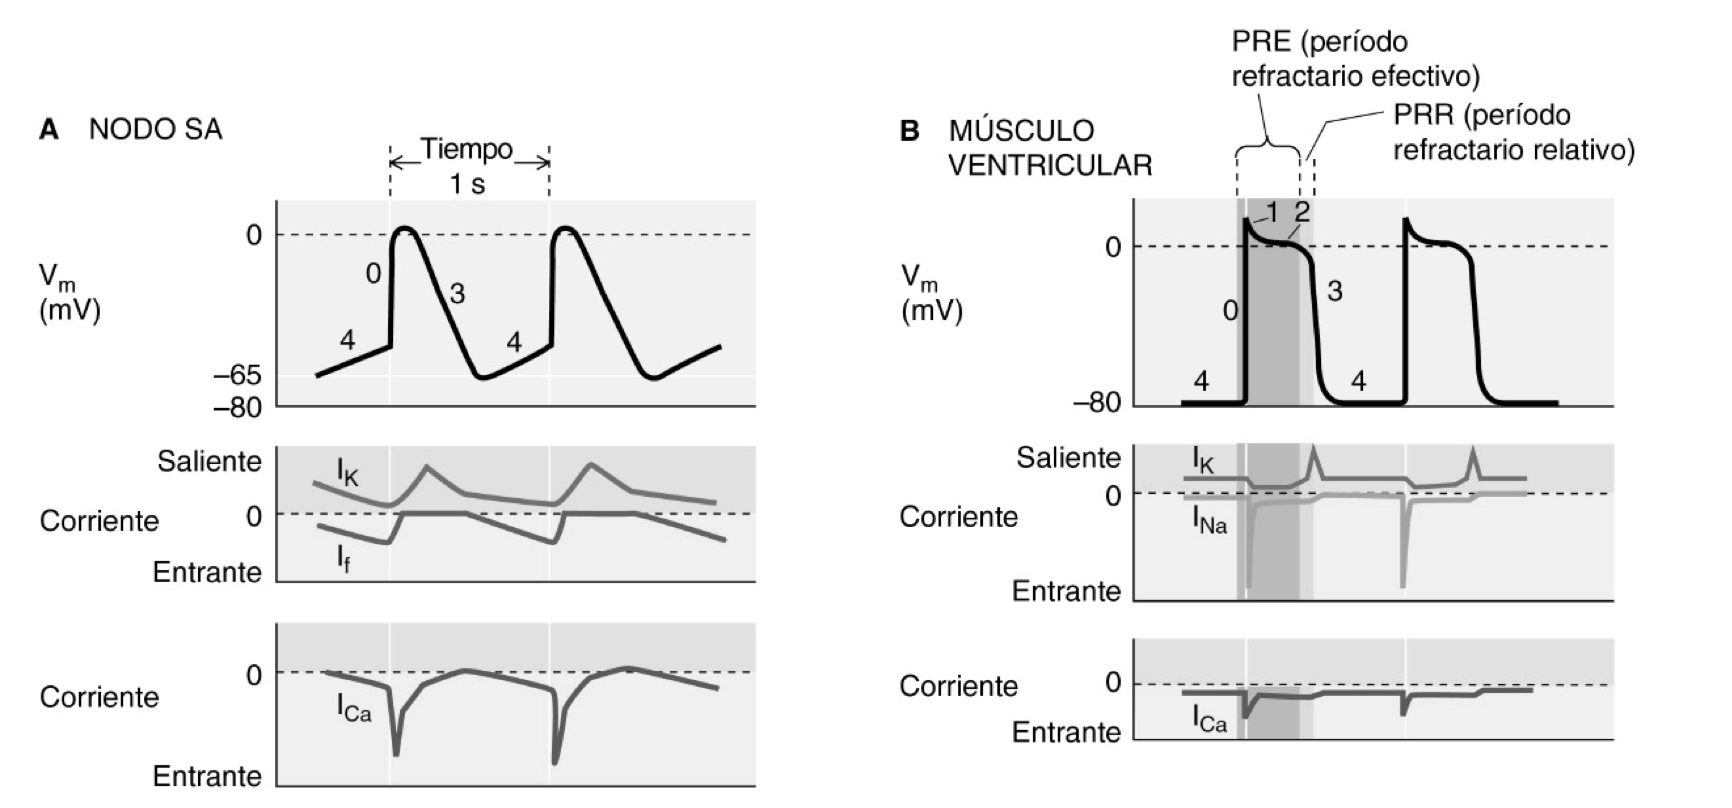
\includegraphics[scale=0.45]{sections/chapter-02/images/action_potential_phases.png}
  \caption[Fases de los potenciales de acción cardíacos.]{Fases de los potenciales de acción cardíacos. Los
  registros de esta figura son ideales. $I_K$, $I_{Na}$, $I_{Ca}$ e $I_f$ son corrientes a través de canales
  de $K^+$, $Na^+$, $Ca^{2+}$ y catiónicos no selectivos, respectivamente. Figura extraída de \cite{bk:boron3ed}}
  \label{fig:action_potential_phases}
\end{figure}

\subsection{Propagación del impulso} \label{subsec:pulse-propagation}

\indent Existen variaciones regionales en la velocidad de conducción del impulso cardíaco. \\
\indent El retardo de conducción no es proporcional a la distancia recorrida, lo cual indica que la velocidad de
propagación no es uniforme. En contraste con el miocardio ordinario y la vía de conducción rápida, los potenciales
de acción de las células nodales presentan menor amplitud y una fase 0 más lenta porque la corriente de $Ca^{2+}$
constituye el elemento predominante de la excitación. El mayor retardo de conducción se observa entre el nódulo AV y
el haz de His, a pesar de que sólo unos pocos milímetros separan a estas dos estructuras. Esto se debe al hecho de
que un potencial lento genera corrientes locales débiles y, por lo tanto, es menos apto para la conducción. Además,
las uniones intercelulares comunicantes o en hendidura son menos numerosas en el nódulo AV. Aunque cada
miocardiocito está rodeada de una membrana aislante, el miocardio se comporta desde el punto de vista eléctrico como
una célula única gigante (sincicio funcional) debido a la presencia de los discos intercalares. Estos discos son
estructuras que separan las células vecinas e incluyen regiones especializadas en las que las membranas adyacentes
se adosan y que contienen "canales" de gran diámetro. Estos permiten el paso de iones y moléculas de bajo peso
molecular y constituyen vías de baja resistencia eléctrica. Estos canales (no selectivos) conducen la corriente del
circuito local, de manera que el flujo eléctrico que parte del nódulo sinusal se propaga a toda la masa del tejido.

\section{Actividad mecánica} \label{sec:mechanical-activity}

El corazón posee una función de bomba, la cual se cumple mediante la contracción y relajación rítmica del músculo
cardíaco que lo forma. Esta formado por dos corazones, el corazón izquierdo y el derecho. El corazón derecho impulsa
sangre venosa que llega luego de haber atravesado los diferentes órganos. Esta desemboca en la aurícula derecha por
dos grandes venas: cava superior y cava inferior. Pasa a través de la válvula tricúspide al ventrículo derecho y
éste la eyecta por la arteria pulmonar al circuito menor; allí se produce la hematosis. La sangre ya oxigenada y con
una presión parcial de dióxido de carbono ($P_{CO_2}$) normal regresa por las venas pulmonares a la aurícula
izquierda. Desde ella pasa a través de la válvula mitral al ventrículo izquierdo, el cual la expulsará por la aorta
a toda la economía. Las válvulas auriculoventriculares, mitras y tricúspide, aseguran la dirección del flujo
sanguíneo al evitar que durante la sístole la sangre que contienen los ventrículos refluya a las aurículas. Las
válvulas sigmoideas, aórtica y pulmonar, también aseguran la dirección del flujo al impedir que la sangre refluya
desde estos vasos a los ventrículos durante el intervalo diastólico. \\
\indent A pesar que los dos ventrículos poseen un volumen interno similar y expulsan igual cantidad de sangre, el
derecho debe generar unos $15-20$ mmHg de presión par abrir la válvula sigmoidea pulmonar, mientars que el izquierdo
debe generar aproximadamente $80$ mmHg para abrir la sigmoidea aórtica. La fuerza que cada uno de estas cavidades
deben hacer explica los grosores de sus paredes. Cada fibra miocárdica realiza la misma fuerza pero el ventrículo
izquierdo posee una mayor cantidad de estas fibras. \\
\indent Los ventrículos de un adulto promedio expulsan aproximadamente $50$ ml por latido. Sin embargo, dejan un
volumen residual sin esxpulsar, que es igual o ligeramente inferior al expulsado. Por lo tanto, el volumen
ventricular antes de la eyección es de unos $70$ a $80$ ml. Este volumen se denomina \textit{volumen diastólico
final} (VDL) y el porcentaje que se expulsa de este volumen se conoce como \textit{fracción expulsada} (FE). Éste es
de aproximadamente $60-70\%$.

\subsection*{Ciclo cardíaco}

El ciclo cardíaco un proceso continuo y periódico, de frecuencia variable de acuerdo a las necesidades del cuerpo
humano. Este ciclo variará su volumen de eyección, su frecuencia cardíaca dependiendo de eventos externos al sistema
cardiovascular. \\
\indent \textbf{Fase isovolumétrica sistólica}. Llamada anteriormente fase isométrica sistólica, pasó
a denominarse isovolumétrica al apreciarse que durante ella se producían cambios en la forma de cavidades, aunque no
en su volumen. El aumento de la presión intrventricular que se origina cuando comienzan a contraerse las fibras
ventriculares origina el cierre de las válvulas auriculoventriculares. Como las válvulas se encuentran cerradas, el
volumen ventricular no se modifica y por este período se denomina isovolumétrico. La presión intraventricular izquierda
asciende desde aproximadamente 20 mmHg a 80 mmHg en menos de una décima de segundo. Esto proporciona una velocidad
media de desarrollo de la presión intraventricular izquierda de alrededor de 700 $\frac{mmHg}{s}$. Cuando las
presiones intraventriculares alcanzan los niveles de las presiones en la aorta o en la arteria pulmonar las válvulas
sigmoideas se abren y esto marca el fin del periódo isovolumétrico. \\
\indent \textbf{Fase de eyección}. Esta fase comienza al abrirse la válvula sigmoidea correspondiente y finaliza al
cerrarse ésta. \\
\indent Durante este período cada uno de los ventrículos eyecta aproximadamente $50-60$ ml. La eyección de la sangre
esta dada por la contracción de las fibras del miocardio. Las presiones medias con las que debe realizar fuerza los
ventrículos son de $100$ mmHg y $16$ mmHg para el el izquierdo y derecho respectivamente. \\
\indent \textbf{Fase isovolumétrica diastólica}. Una vez que la expulsión finaliza, y que la presión en la aorta o
la pulmonar iguala o supera a la existente en el ventrículo izquierdo o el derecho, las válvulas sigmoideas se
cierran. Como las válvulas auriculoventriculares aún permanecen cerradas, la presión intraventricular disminuirá sin
cambios de volumen. La presión descenderá de forma isovolumétrica hasta que la presión en las aurículas supere a la
ventricular y se abran las válvulas auriculoventriculares. \\
\indent \textbf{Fase de llenado}. La apertura de las válvulas auriculoventriculares señala el inicio de la fase de
llenado, la cual se complementará con la contracción auricular, la cual dará por finalizado a esta fase.

\indent En la Figura \ref{fig:cardiac_cycle} se ilustra el ciclo cardíaco en un gráfico de presión-volumen donde
queda definido claramente los diferentes hitos del ciclo.

\begin{figure}[H]
  \centering
  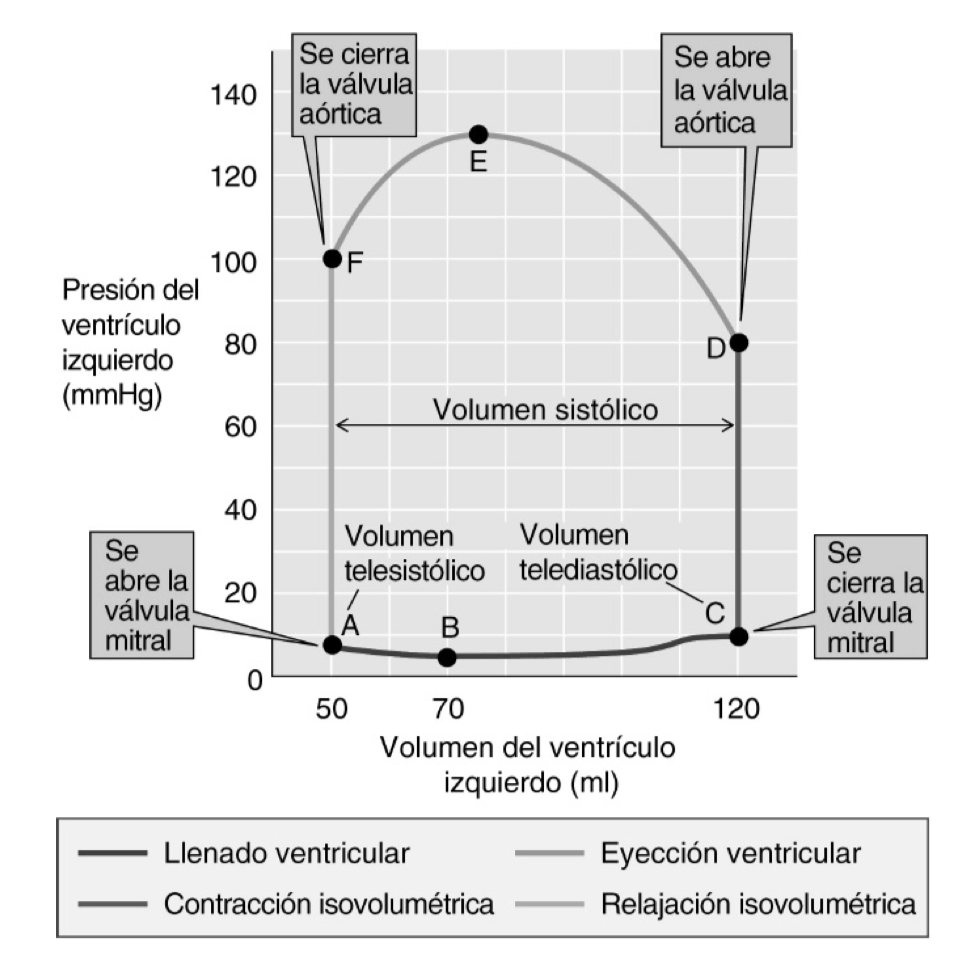
\includegraphics[scale=0.65]{sections/chapter-02/images/cardiac_cycle.png}
  \caption[Curva de presión-volumen del ventrículo izquierdo.]{Curva de presión-volumen del ventrículo izquierdo.
  Figura extraída de \cite{bk:boron3ed}}
  \label{fig:cardiac_cycle}
\end{figure}

\section{El Fonocardiograma} \label{sec:the-phonocardiogram}

La actividad mecánica del corazón genera movimientos vibratorios en las diferentes estructuras cardíacas que se
propagan hacia la superficie torácica. Algunas de esas vibraciones son identificadas por el oído humano y
constituyen los ruidos cardíacos. Los movimientos vibratorios de menor frecuencia, detectados por la
visualización o por la palpación de expansiones o retracciones en determinadas regiones de la superficie,
configuran los diferentes pulsos.

\subsection{Ruidos cardíacos} \label{sub:cardiac-sounds}

En toda la superficie torácica próxima al corazón se auscultan dos ruidos cardíacos, definidos como el primero
($1^o$) y el segundo ($2^o$) ruido. Éstos coinciden con el comienzo y el final de la sístole ventricular,
respectivamente, y brindan una idea secuencial de los fenómenos que ocurren durante el ciclo cardíaco. Con menor
frecuencia se pueden auscultar otros dos ruidos que se reconocen como tercero ($3^o$) y cuarto ($4^o$). \\
\indent \textbf{Primer ruido}. El primer ruido cardíaco se produce por movimientos vibratorios generados en las
válvulas auriculoventriculares (mitral y tricúspide) y en las estructuras próximas a ellas. Las vibraciones tienen
lugar en el momento del cierre valvular y coinciden con el comienzo de la contracción ventricular o sístole
ventricular. \\
\indent En este ruido predominan vibraciones de baja frecuencia que le confieren una característica auditiva
grave. \\
\indent La zona donde se ausculta mejor y se obtiene el mejor registro gráfico del primer ruido es la región
próxima a la punta del corazón y el área correspondiente a la base del esternón. \\
\indent El registro gráfico de ese ruido (intensidad de la frecuencia vibratoria en función del tiempo),
conocido como fonocardiograma, muestra un grupo central de vibraciones con frecuencia vibratoria de 120 a 142 Hz,
precedido y seguido por movimientos vibratorios de frecuencias menores, entre 30 y 100 Hz. El primer ruido tiene una
duración promedio de $0.1-0.12$. \\
\indent \textbf{Segundo ruido}. Al cerrarse las válvulas aórtica y pulmonar se generan movimientos vibratorios
que determinan la generación del $2^o$ ruido. La conformación anatómica de esas estructuras le da al segundo ruido
características auditivas diferentes: su duración es menor, entre $0.07-0.10$ s y frecuencias entre $150-170$ Hz. \\
\indent Por razones de proximidad topográfica, y si bien se puede identificar en toda la región anterior del
tórax, el sitio donde se ausculta y registra mejor es a nivel del segundo espacio intercostal, tanto a la izquierda
del esternón como a la derecha.
\indent \textbf{Tercer ruido}. El tercer ruido cardíaco es auscultado en casi todos los niños y adolescentes sin
enfermedad cardíaca; su prevalencia auscultatoria es menor a medida que aumenta la edad en individuos sanos (23\% en
una población de ambos sexos entre 36 y 37 años de edad). \\
\indent La presencia de este rudio está directamente vinculada a las vibraciones de la pared ventricular durante
el llenado ventricular rápido. \\
\indent \textbf{Cuarto ruido}. El cuarto ruido, también de auscultación poco frecuente en adultos sanos,
coincide con la última parte del llenado ventricular, secundaria a la contracción auricular. Es precedido por la
onda P del registro del electrocardiograma y sigue inmediatamente la contracción auricular. Esto se puede observar
en la Figura \ref{fig:diagrams_in_phase}.

\begin{figure}[H]
  \centering
  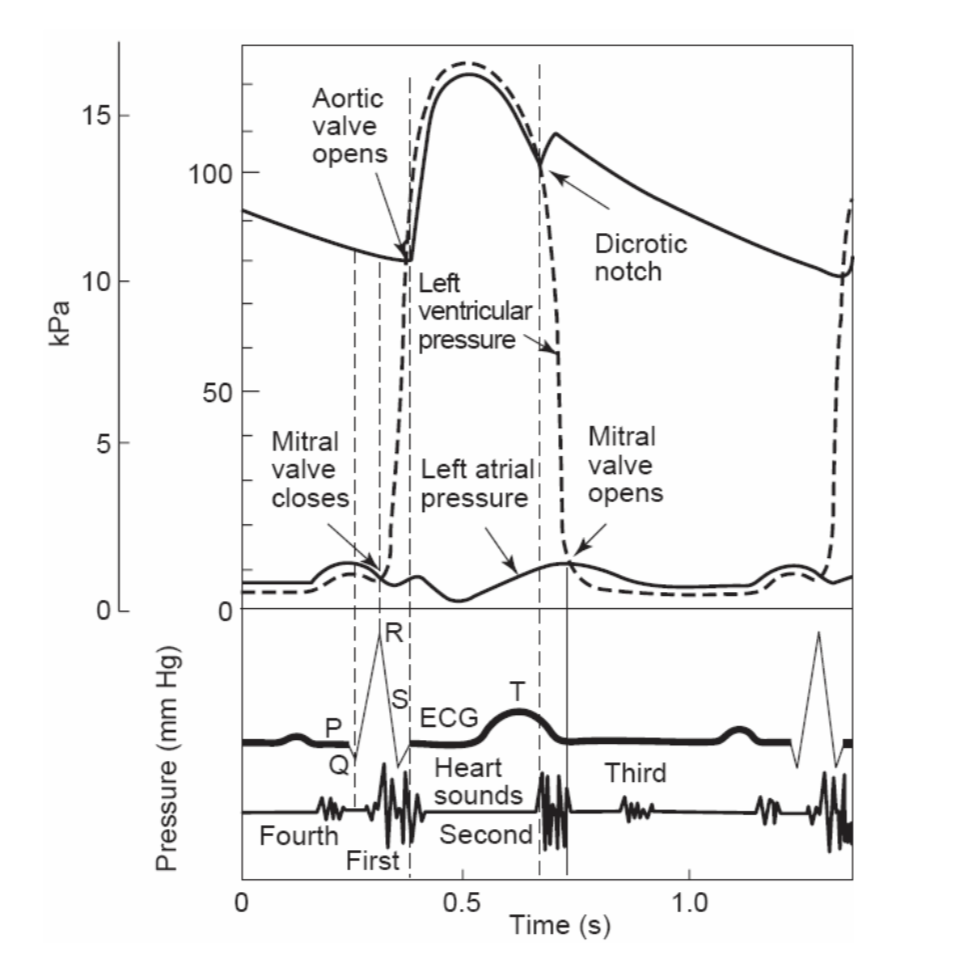
\includegraphics[scale=0.65]{sections/chapter-02/images/diagrams_in_phase.png}
  \caption[Correlación de los cuatro sonidos cardíacos con los eventos eléctricos y mecánicos del
  cíclo cardíaco en fase.]{Correlación de los cuatro sonidos cardíacos con los eventos eléctricos y
  mecánicos del cíclo cardíaco en fase. Figura extraída de \cite{pp:abbas2014}.}
  \label{fig:diagrams_in_phase}
\end{figure}

\indent El Cuadro \ref{tab:cardiac_sounds} resume los tipos y las características de los ruidos cardíacos. La
identificación de los ruidos cardíacos normales que determinan la sístole y la diástole es la base de la
auscultación. Dicho esto, resulta de suma importancia tener perfectamente caracterizada a la señal que surge de la
auscultación o fonocardiografía.


\begin{table}[H]
  \centering
  \begin{tabular}{ |llll| }
    \hline
    \thead{RUIDO} & \thead{LOCALIZACIÓN \\ EN EL CICLO \\ CARDÍACO}  & \thead{MECANISMO}  & \thead{IMPLICACIÓN
    \\ CLÍNICA}  \\
    \hline
    \thead{4$^{to}$ ruido} & \thead{Presistólico, antes del \\ 1$^{er}$ ruido} & \thead{Contracción enérgica \\
    de aurícula} & \thead{Patológico, HTA, \\ alteración de la \\ distensibilidad del \\ VI o del VD} \\
    \thead{1$^{er}$ ruido} & \thead{Inicio de la \\ sístole ventricular} & \thead{Cierre de válvulas AV} &
    \thead{Fisiológico si \\ es normal} \\
    \thead{Clics \\ mesotelesistólicos} & \thead{Mesotelesistólicos} & \thead{Desplazamiento posterior \\ hacia
    aurícula \\ de valvas mitrales \\ (posterior)} & \thead{Patológicos. \\ Aislados o antes \\ de soplos
    sistólicos \\ por insuficincia \\ mitral}\\
    \thead{2$^{do}$ ruido} & \thead{Fin de la sístole} & \thead{Cierre de válvulas \\ sigmoideas, aórtica y \\
    pulmonar} & \thead{Fisológico \\ si es normal} \\
    \thead{Chasquidos de \\ apertura} & \thead{Inicio de la diástole, \\ después del 2$^{do}$ ruido. \\ Inicio
    de la sístole, \\ después del 1$^{er}$ ruido} & \thead{Apertura de la \\ válvula AV enferma \\ (reumática),
    aperturas \\ sigmoideas enfermas} & \thead{Patológicos. Estenosis \\ mitral y tricuspídea. \\ Estenosis
    aórtica y \\ pulmonar} \\
    \thead{3$^{er}$ ruido} & \thead{Protodiastólico} & \thead{Distensión ventricular súbita \\ en la fase de
    llenado rápido} & \thead{Fisiológico en niños \\ y adultos jóvenes. \\ Patológico en el resto.} \\
    \hline
  \end{tabular}
  \vspace{0.5ex}
  \raggedright \textit{\footnotesize VI: Ventrículo Izquierdo; VD: Ventrículo derecho; HTA: Hipertensión
  arterial; AV: auriculoventricular.}
  \caption{Tipos y características de los sonidos cardíacos.}
  \label{tab:cardiac_sounds}
\end{table}

\subsection{Estado del arte} \label{subsec:state-of-the-art}

A partir de esto surgieron propuestas de procesar, clasificar y segmentar las señales derivadas del
fonocardiograma. El PCG es una onda mecánica, particularmente sonido, que refleja el proceso del corazón como
bomba cardíaca y en ella queda asentado el correcto funcionamiento del corazón, esto ya sea las válvulas
cerrándose correctamente, el ritmo cardíaco, rigidez de las paredes cardiovasculares, entre otras
características. \\
\indent Aquí surgen varios desafíos. La clasificación de patologías cardíacas asociadas y segmentación de la
señal en sus sonidos fundamentales. Todo esto en la práctica, al realizar la adquisición de estas señales se
encuentra contaminado de distintos factores, externos al fonocardiograma. Estas fuentes de ruido pueden ser de
naturaleza eléctrica, como la tensión de línea de $50-60$ Hz (dependiendo de la zona geográfica) o mecánica como el
habla. Otros ejemplos contaminación es la respiración (de baja frecuencia), produce que la línea isoeléctrica se
perciba como oscilante. Por otro lado, puede haber presencia de ruido muscular. \\
\indent Hasta la actualidad varias personas han trabajado con estos problemas, ya sea tanto clasificación como
segmentación. Liang et al. en \cite{pp:liang}, han trabajado con algoritmos determinísticos basados en la detección
de picos con la energía y envolvente de Shannon. Esto ha mostrado una performance interesante pero ante señales muy
corruptas puede haber picos que interfieran con la detección y reduzcan la eficiencia de detección de los sonidos
fundamentales. Luego, un segundo trabajo en \cite{pp:liang2} se utilizó la descomposición de wavelet y la energía de
Shannon para detectar los picos en cada bloque y realizar la segmentación, así obteniendo una vez más performance
altas aunque similares al trabajo anterior. \\
\indent En 2010, Schmidt \textit{et al.} \cite{pp:schmidt2010} han propuesto un sistema de segmentación donde
proponen el algoritmo \acrshort{dhmm} (\textit{Duration-dependant Hidden Markov Model}) logrando un alto desempeño a
la hora de la clasificación de los sonidos fundamentales tanto para pacientes sanos como enfermos. Luego, en 2014,
Abbas \textit{et al.} \cite{pp:abbas2014} han propuesto una técnica de clasificación basada en \textit{K-means
clustering} mostrando una alta estabilidad en la detección y clasificación, donde juega un rol vital en la
cuantificación e identificación de diferentes casos hemodinámicos. Hasta 2015, los distintos métodos de clasificación
debían estar acompañadas por señales adicionales como el ECG. En 2015, David Springer \textit{et al.}
\cite{pp:springer2015} han publicado un algoritmo de segmentación de los sonidos S1 y S2 con un sólo canal de PCG
sin referencia externa usando una modificación del algoritmo propuesto por Schmidt, así mejorando la perfomance del
estado del arte. \\
\indent Recientemente, Franceso Renna y Miguel Coimbra de la Universidad de Porto, Portugal, propusieron el uso
de \acrshort{cnn} (\textit{Convolutional Neural Network}). Este enfoque fue utilizado en otros trabajos para la
segmentación de imágenes. Asimismo, aplicaron a la salida de diferentes modelos temporales que generan una salida
consistente y que responde a la naturaleza de transición de los estados del fonocardiograma, mejorando las métricas
del trabajo de Springer.
    